\chapter{Experiments}
\label{chap:4}

% - debug plotting
% -- acq func plots
% -- hyper opt plots

\section{Cart Pole}

% \begin{wrapfigure}{R}{0.3\textwidth}
%     \centering
%     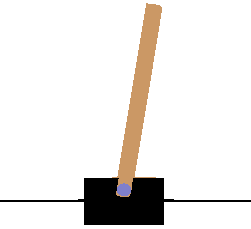
\includegraphics[width=0.29\textwidth]{/home/sebastian/Documents/bscThesis/img/cartpole.pdf}
%     \caption{Visualization of the Cart Pole rendered by the OpenAI Gym\label{fig:cartpolePygym}}
% \end{wrapfigure}

% \begin{figure}[h]
%     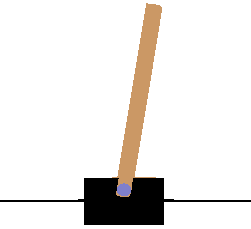
\includegraphics{/home/sebastian/Documents/bscThesis/img/cartpole.pdf}
%     \caption{Visualization of the Cart Pole rendered by the OpenAI Gym\label{fig:cartpolePygym}}
% \end{figure}

The Cart Pole environment consists of a cart with a pole attached to its top. The cart is accelerated to the left or the right to balance the pole for as long as possible. An episode starts with small random state values and it ends when the maximum of time steps or a specific state is reached. The state values contain the position and the velocity of the cart, and the angle and the angular velocity of the pole. Each of these four state values are set uniformly random between -0.05 and 0.05 at the beginning. The episode ends after 200 time steps or if the pole falls below 12 degrees relative to the vertical. It also ends when the cart is more than 2.4 meters away from the center. For each completed time step a reward of 1 is returned. The cart pole implementation from OpenAI Gym ('CartPole-v0') accepts a discrete action value, -1 or 1, for either applying force to the left or to the right. With the four state values and an additional bias value we have five dimensions for each discrete action resulting in a total of ten dimensions. In our own cart pole simulation, we only use the four state parameters for calculating an continuous action value between -1 and 1. It turned out that adding a bias value would make the policy search slightly more difficult here. Therefore, this policy has only four dimensions. Also we let an episode end after a maximum of 1000 timesteps.


% \begin{figure}
% \centering
% \begin{minipage}{.5\textwidth}
%   \centering
%   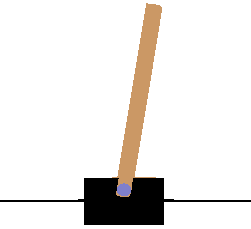
\includegraphics[width=.49\linewidth]{/home/sebastian/Documents/bscThesis/img/cartpole.pdf}
%   \captionof{figure}{Visualization of the Cart Pole rendered by the OpenAI Gym}
%   \label{fig:cartpolePygym}
% \end{minipage}%
% \begin{minipage}{.5\textwidth}
%   \centering
%   
\includegraphics[width=.49\linewidth]{/home/sebastian/Documents/bscThesis/img/acrobot.pdf}
%   \captionof{figure}{Visualization of the Acrobot rendered by the OpenAI Gym}
%   \label{fig:acrobotPygym}
% \end{minipage}
% \end{figure}

\section{Acrobot}

% \begin{figure}[h]
%     
\includegraphics[width=0.20\textwidth]{/home/sebastian/Documents/bscThesis/img/acrobot.pdf}
%     \caption{Visualization of the Acrobot rendered by the OpenAI Gym\label{fig:acrobotPygym}}
% \end{figure}

% \begin{wrapfigure}{R}{0.3\textwidth}
%     \centering
%     
\includegraphics[width=0.29\textwidth]{/home/sebastian/Documents/bscThesis/img/acrobot.pdf}
%     \caption{Visualization of the Acrobot rendered by the OpenAI Gym\label{fig:acrobotPygym}}
% \end{wrapfigure}

The Acrobot consists of two joints and two pendulums. The upper joint has a fixed position. It connects to the first pendulum, which is attached to the second joint. A torque can be applied to that second joint, which controls the second pendulum. The pendulums start in equilibrium position and the goal is to gain enough momentum and swing the end of the second pendulum above a certain mark. If the Acrobot passes that mark, the episode ends. A reward of -1 is received for every timestep needed. The angle between vertical and the first pendulum and the angle between the two pendulums form the six state parameters. Four parameters are the sine and the cosine of these two angles each, whereas the last two parameters are the angular velocities \ref{table:envs}. The discrete action can have the values -1, 0 or 1. Each value stands for the amount of torque applied to the joint between the two pendulum links. With the six state values, an additional bias value, and three discrete action possibilities we get 21 dimensions for the Acrobot policy. We use the OpenAI Gym implementation of Acrobot ('Acrobot-v1').

\section{Mountain car continuous}

% \begin{wrapfigure}{R}{0.5\textwidth}
%     \centering
%     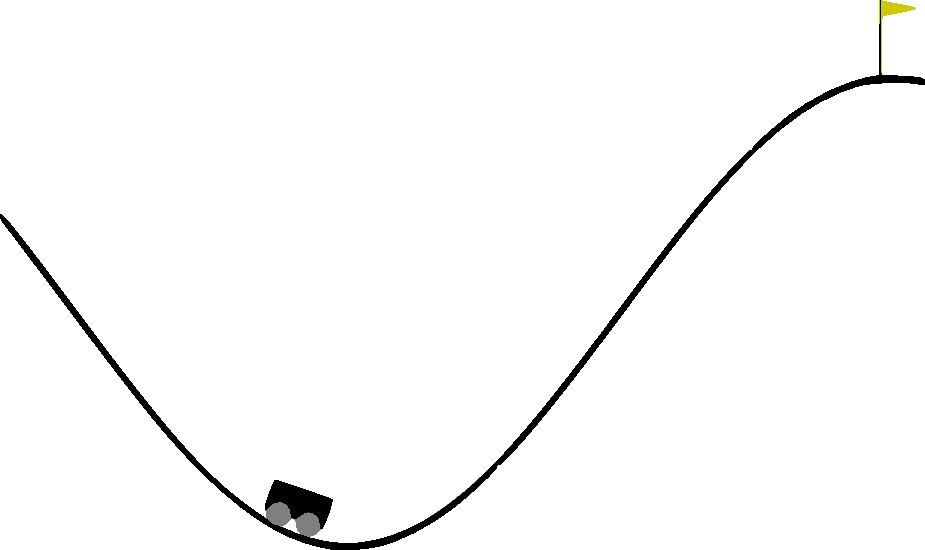
\includegraphics[width=0.45\textwidth]{/home/sebastian/Documents/bscThesis/img/mountaincar.pdf}
%     \caption{Visualization of the mountain car rendered by the OpenAI Gym\label{fig:mountaincarPygym}}
% \end{wrapfigure}

During the Mountain Car task, an underpowered car tries to drive uphill. It can only reach the goal on the right side if it uses both hills to gain momentum. The end of the left hill is an inelastic wall, so if the car hits it, the velocity is set to zero. In the continuous setup the reward starts at 100. After an episode the squared count of performed actions is subtracted. Since the hills are formed by a sine curve, it is sufficient that the position of the car is only one-dimensional. The vertical position of the vehicle can be easily derived from the horizontal position with the sine function. The horizontal position and the car's velocity are cubically expanded (Table \ref{table:envs}) to get nine state values. Also a bias parameter is added as a tenth state value. In the continuous setting, we therefore receive ten dimensions. We use the OpenAI Gym implementation of the continuous Mountain Car task ('MountainCarContinuous-v0').

%In the discrete setting we have three action values for either applying acceleration to the left or right (-1,1) or doing nothing (0). In this case we receive 30 dimensions.



%
% \begin{figure}
%     \begin{center}
%         \fbox{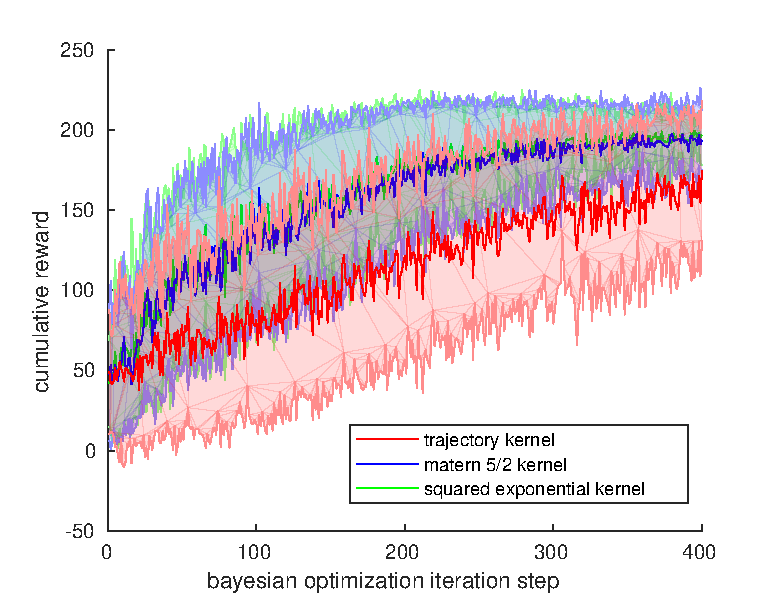
\includegraphics{/home/sebastian/Documents/bscThesis/img/cartpole_matlab_conti_newreward_local}}
%         \caption{Local opt, 4 dim. Mean and standard deviation from 32 trials of each kernel. Cartpole matlab implementation with new reward function, 200 timesteps, and continuous action selection.}
%     \end{center}
% \end{figure}
%
% \begin{figure}
%     \begin{center}
%         \fbox{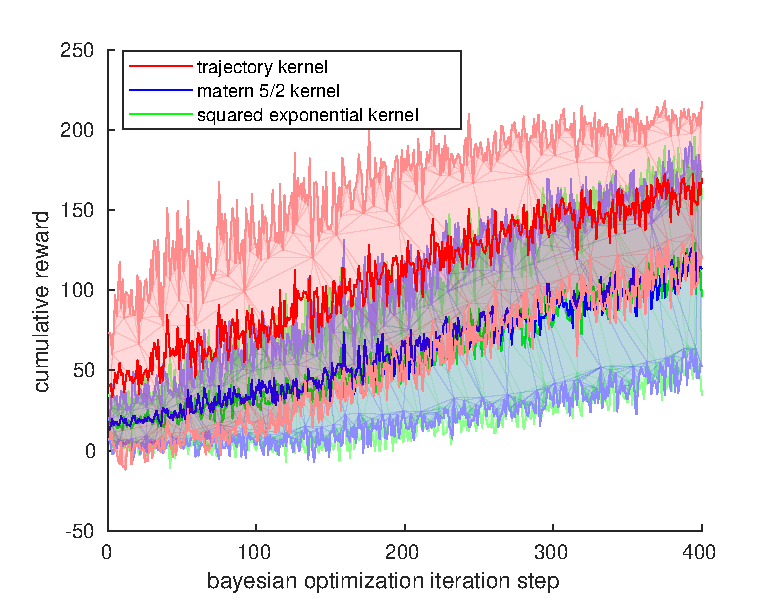
\includegraphics{/home/sebastian/Documents/bscThesis/img/cartpole_pygym_disc_local}}
%         \caption{Local opt, 10 dim. Mean and standard deviation from 32 trials of each kernel. Cartpole python gym implementation, 200 timesteps, and discrete action selection.}
%     \end{center}
% \end{figure}

\begin{table}[h]
    \begin{tabularx}{\textwidth}{ |l|X|l|X|l|l| }
    \hline
    Environment & Description & Action & State feature & \# dimensions & Platform \\ \hline
    Cart Pole & $p$: \tabto{16pt} cart position \newline
                $\theta$: \tabto{16pt} pole angle & continuous: [-1,1] & $(p,\dot{p},\theta,\dot{\theta})$ & 4 & MATLAB\\ \cline{3-6}
     &  & discrete: \{-1,1\} & $(p,\dot{p},\theta,\dot{\theta},1)$ & 10 & OpenAI Gym\\ \hline
    Acrobot & $\theta_1$: \tabto{16pt} angle of \tabto{16pt} pendulum 1 \newline $\theta_2$: \tabto{16pt} angle between \tabto{16pt} pendulum 1 and \tabto{16pt} 2 & discrete: \{-1,0,1\} & (\tabto{4pt}$\cos(\theta_1), \sin(\theta_1),$\tabto{4pt}$\cos(\theta_2), \sin(\theta_2),$\tabto{4pt}$\dot{\theta_1}, \dot{\theta_2}, 1)$ & 21 & OpenAI Gym\\ \hline
    Mountain Car & $p$:\tabto{16pt}horizontal car \tabto{16pt} position \newline $u$: \tabto{16pt} car velocity & continuous: [-1,1] & $(p, u, p^2, u^2, p u, p^2 u,$\tabto{4pt}$p u^2, p^3, u^3 , 1)$ & 10 & OpenAI Gym\\ \cline{3-6}
    & & discrete: \{-1,0,1\} & $(p, u, p^2, u^2, p u, p^2 u,$\tabto{4pt}$p u^2, p^3, u^3 , 1)$ & 30 & OpenAI Gym\\ \hline
    \end{tabularx}
    \caption{Environment parameters of the experiments\label{table:envs}}
\end{table}

\begin{figure}[h]
    \centering
    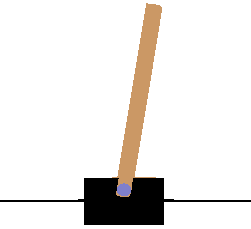
\includegraphics[width=.24\textwidth]{/home/sebastian/Documents/bscThesis/img/cartpole.pdf}
    
\includegraphics[width=.24\textwidth]{/home/sebastian/Documents/bscThesis/img/acrobot.pdf}
    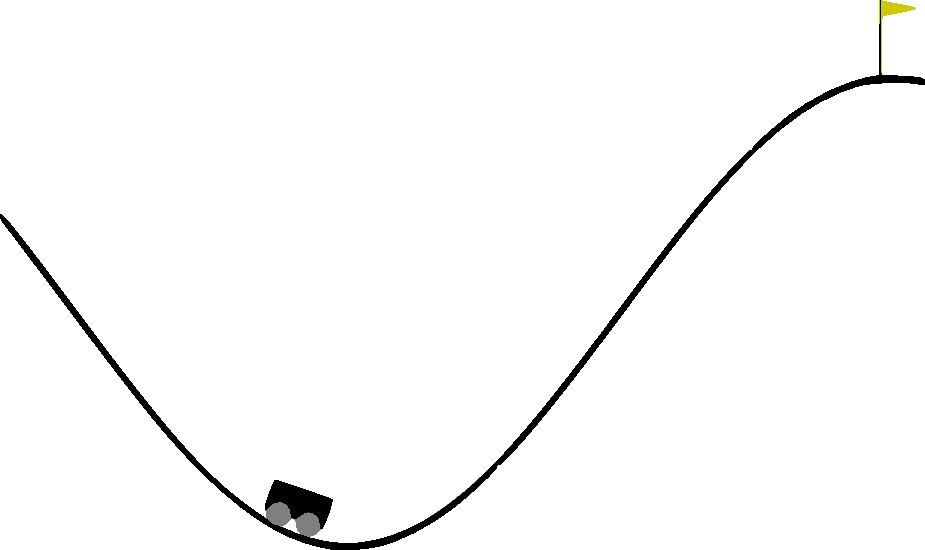
\includegraphics[width=.49\textwidth]{/home/sebastian/Documents/bscThesis/img/mountaincar.pdf}

    \caption{BLABLABLAH}
    \label{fig:cartpoleacrobot}
\end{figure}

\section{Implementation of the environments}

Since we developed the Bayesian optimization algorithm in MATLAB, we first implemented a MATLAB version of Cart Pole that was adapted from \cite{joseCode}. Then we also implemented the OpenAI Gym \cite{DBLP:journals/corr/BrockmanCPSSTZ16} to provide a wide range of problem environments. To use the simulations written in Python we prepared a python module which is imported to MATLAB. After loading the python module with \verb|py.importlib.import_module(moduleName)| we can call every method it contains via the \verb|py.moduleName.| prefix. It is vital to convert our MATLAB data correctly before calling the python subroutine with it. The MATLAB variables containing whole numbers are converted from \verb|Double| to \verb|Int|. Also all the vectors received by the python module have to be converted to an array through \verb|numpy.asarray()|.

To cut the time for experiment runs we vectorized every suited operation to speed up calculations in MATLAB. In addition, we tuned the code to run on a parallel pool so we could run experiments on the cluster efficiently. Unfortunately, the OpenAI Gym environments do not work if we use the parallelization of MATLAB. So we used these environments only with the less computationally demanding local Bayesian optimization.\\

% \subsection{Global optimization}
% The expected improvement function and the log marginal likelihood function for hyper parameter optimization need to be maximized. Since we use MATLAB's \texttt{GlobalSearch} Toolbox, which is a global minimizer, we multiply the results of the functions by -1 to be able to minimize them appropriatly.
% \\
% % When optimizing the expected improvement function or the hyper parameter space we use the \texttt{GlobalSearch} Toolbox from MATLAB. But if we run the experiments on the cluster we use the local optimizer \texttt{fmincon} on 10000 random starting points to work around the lack of free global optimization toolbox licences.
%
% \subsection{Optimization starting point}
% When optimizing the log marginal likelihood of the Gaussian process we are confronted with undefinded areas in the hyper parameter space because $K$ is not positive semi definit in those areas. To start the optimization properly we randomly select points until finding a defined one.

\section{Action selection}
\label{sec:actionselection}
In continuous action space we use a linear policy to action mapping
\begin{equation} \label{eq:actionselection}
    a = f_s(s)^\top x + \sigma_a,
\end{equation}

with a small Gaussian noise $\sigma_a$ needed for stochastic policies. So the Gaussian distributed actions,

$$a \sim \mathcal{N}(f_s(s) x,\sigma_a^2),$$

result in the probability measure by the Gaussian density:

\begin{equation}\label{eq:contiAS}
    P_{\pi}(a|s,x) = \frac{1}{\sqrt{2\pi\sigma_a^2}}\exp\left(-\frac{(a-f_s(s)x)^2}{2\sigma_a^2}\right).
\end{equation}

In discrete action space environments we use a parametric soft-max action selection policy:

\begin{equation} \label{eq:discreteactionselection}
    P(a|s,x)= \frac{\exp(f_s(s)^\top x_a)}{\sum_{a\in A} \exp(f_s(s)^\top x_a)}.
\end{equation}

Again it consists of the linear mapping $f_s(s)^\top x$, and $A$ holds all possible actions. The resulting action is then sampled from the probability of action $a$ given state $s$.

The state feature function $f_s(s)$ depends on the environment as listed in Table \ref{table:envs}.

\section{Initial settings}

For the trajectory kernel, we proposed in section \ref{sec:ownTK}, a maximum of 500 random states as the subset $S_{\text{sub}}$ are used.

For the continuous action selection the standard error deviation $\sigma_a$ is set to $10^{-3}$. We adapted the action selection strategies from \cite{wilson2014using}. Unfortunately, they do not provide any parameters. Therefore this error deviation value was guessed after a few test runs.

The noise variance $sigma_n^2$ is set to $10^{-8}$ for all performance tests.

\subsection{Global context}

In the global search context the policy parameter boundaries are set to -10 and 10 for each dimension resulting in a $d$ dimensional hypercubic search space.

For the Bayesian optimization we select the initial samples set $X_n$ from a bunch of sample sets such that the Euclidean distance between points of the selected set is maximized. This grants us a well covered search space as a starting condition. We also set the number of initial samples to $M = 10$ and the iteration count to $N = 200$.

In the expected improvement function, the trade-off parameter $\tau$ is set to 0.01 as proposed by \cite{brochu2010tutorial}.

The hyper parameter optimization runs every fifth Bayesian optimization step or if the maximum of the expected improvement function drops below $10^-6$.

\subsection{Local context}
% -- fmincon local search on distance covariance
The Bayesian optimization in the local context starts with a hypersphere centred at the origin with radius 10 as the policy search space boundary. The starting point for the search is set to the origin accordingly.

We run the hyper parameter optimization every time the search space is adjusted. We carry out a total of 400 Bayesian optimization steps, in which the search space is adapted every four steps.

Before doing Gaussian process regression we transform our observations to zero mean and uniform variance:
$$y = \frac{y_{n}-\mathrm{mean}(y_{n})}{\mathrm{std}(y_{n})}.$$
This standardization proposed by \cite{akrour2017local} affects the Thompson sampling exploration exploitation trade-off. The distance threshold $d_t$ (algorithm \ref{alg:acqLocalBO}) for the samples during Thompson sampling is set to 80\%.
